
\section{Conclusion}


%Give a concise summary of your research and finding here, and include a short summary of any future work as well.

The goal of this project was to create a full-stack web application for managing the configuration of distributed software environments. We aimed to provide a user-friendly interface that minimizes potential misconfiguration and human errors. \\

\noindent
To meet the project requirements, we designed the application as a containerized solution that can be deployed on Kubernetes. We used React with Next.js as the framework for the front-end, Prisma as the ORM solution, and Chakra UI as the component library. Our back-end was built with tRPC, providing end-to-end type-safe API code. Docker was used for containerization. \\

\noindent
Despite successfully meeting our minimum requirements, we had to make certain compromises due to time constraints. As a result, we were unable to fully develop some of our envisioned features for the configuration browser. However, we are overall satisfied with the results achieved in this project. Given that we were unable to find any existing solutions for a problem like this, we are pleased with what we have accomplished. \\

\section{Limitations and future work}

\subsection{Prisma cold start time}

Serverless computing platforms, such as Vercel, have the benefit of scaling automatically based on traffic and usage, but they also have the limitation of experiencing a cold start when a new request comes in. This means that the server needs to initialize and allocate resources before it can start processing the request, which can add a delay to the response time. It's worth noting that once the server is initialized, it can process subsequent requests more quickly without incurring the same initialization delay. This being a serverless platform, the server has a set lifetime before it gets despawned, which allows it to handle multiple requests within that time frame without incurring the cold start delay again. \\

\noindent
In our project, we use Prisma as our ORM to interact with the database. Prisma currently uses a protocol based on GraphQL, which adds a considerable CPU and memory overhead that can further slow down the cold start time. To improve this, the Prisma team has recently created a new JSON-based wire protocol that eliminates GraphQL and can improve startup times by up to 9 times on large schemas. \\

\noindent
This new protocol is more efficient mainly because it no longer requires the DMMF (Data Model Meta Format) to serialize messages, the Rust runtime that was used for running GraphQL was dropped, among other optimizations. It is worth noting that the protocol itself is not just JSON but rather a JSON-based wire protocol. \cite{prisma_JSON_protocol} \\

\noindent
This feature is still in preview and won't be ready for production until after the completion of this thesis. However, we were able to test the performance benefits of this new protocol. We took five measurements of the cold start time, plotted them and calculated the average start time. We found that this new protocol improves the start times by around $\approx 62\%$ in our case, reducing the cold start wait time from around 8 seconds to roughly 3. The results that are included in  \autoref{table:prisma_before_after} and the mean time in \autoref{figure:prisma_before_after}, show a significant improvement in cold start performance after the introduction of the new protocol. \\

\begin{table}[ht]
\centering
\begin{tabular}{lrlrl}
        & \multicolumn{1}{l}{Before} &   & \multicolumn{1}{l}{After} &   \\ \cline{2-5}
        & 8.84                       & s & 2.58                      & s \\
        & 7.95                       & s & 3.02                      & s \\
        & 7.82                       & s & 2.30                       & s \\
        & 8.31                       & s & 3.94                      & s \\
        & 8.41                       & s & 3.92                      & s \\ \cline{2-5} 
Average & 8.27                       & s & 3.15                      & s
\end{tabular}
\caption[Prisma serverless cold start tests]{Comparison of Prisma serverless cold start times before and after the introduction of the new JSON-based wire protocol. The start times of the five measurements are shown in seconds.}
\label{table:prisma_before_after}
\end{table}

\begin{figure}[h]
\centering
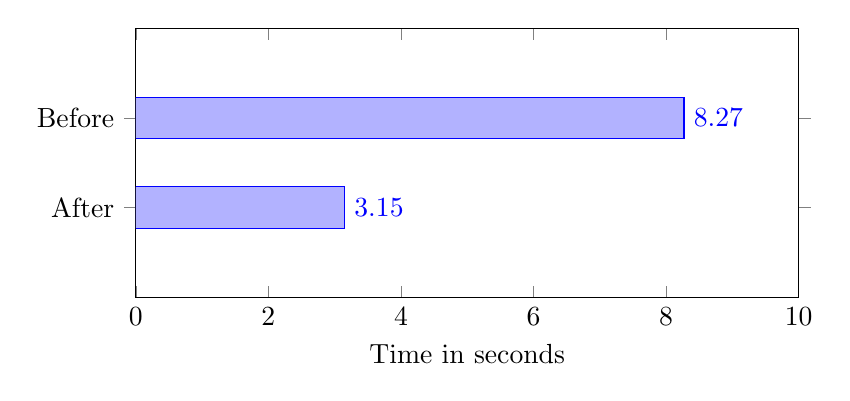
\begin{tikzpicture}
\begin{axis} [
    xbar,
    ytick={1,2},
    yticklabels={After, Before},
    xlabel=Time in seconds,
    % ylabel=Mean,
    xmin=0, xmax=10, ymin=0, ymax=3,
    height=5cm, width=10cm,
    nodes near coords,
    bar width=15pt
]
\addplot coordinates {
    (3.15, 1)
    (8.27, 2) 
};
\end{axis}
\end{tikzpicture}
\caption[Prisma cold start mean time]{The comparison of mean start times before and after the introduction of the JSON protocol}
\label{figure:prisma_before_after}
\end{figure}


\subsection{Upgrading Next.js}

Upgrading to a newer Next.js version would bring several improvements to our application. This latest version brings a range of enhancements that can significantly benefit our project. One notable improvement is the update to React 18+, which introduces advancements in concurrent rendering, streaming from server components, and automatic batching of state changes, among other out-of-the-box enhancements. \cite{react_blog_reactv18} This upgrade would allow us to leverage the latest features and optimizations provided by React, leading to improved performance and a smoother user experience. \\

\noindent
Next.js 13.4 also stabilizes the App Directory feature, which brings substantial improvements to the file system-based router and facilitates the creation of complex layouts with advanced routing patterns. \cite{nextjs_blog_next13} This feature provides a more streamlined and efficient approach to managing routes, enhancing the overall architecture of our application. \\

\noindent
Additionally, Next.js 13 introduces Turbopack, a new Rust-based Webpack replacement. According to the creators of Vercel, Turbopack can deliver a performance boost of up to 700x compared to traditional Webpack. \cite{nextjs_turbopack} This upgrade would result in improved image optimization, enhanced font management, and a more efficient link component, further optimizing the loading and rendering speed of our application. \\

